\chapter{YOLO: You Only Look Once}
You only look once (YOLO) \cite{yolo} is a state-of-the-art, real-time object detection system. It is regression based object detection algorithm which has very high speed with reasonable trade-off of accuracy. Previously, object detection was considered as a classification problem, YOLO algorithm is the first proposed method which solved it as a regression problem and set a new ground for object detection. 

\section{Introduction}
The human visual system is fast and accurate, allowing us to perform complex tasks like driving with little conscious thought. Fast, accurate algorithms for object detection would allow computers to drive cars without specialized sensors, enable assistive devices to convey real-time scene information to human users, and unlock the potential for general purpose, responsive robotic systems.

Current detection systems like DPM \cite{dpm}(Deformable Part Model), R-CNN, Fast R-CNN \cite{fast_rcnn} solve object detection as a classification problem in multiple steps which is time consuming and cannot be optimized for well. YOLO re-frames object detection as a single regression problem, straight from image pixels to bounding box coordinates and class probabilities.

YOLO is refreshingly simple. A single convolutional network simultaneously predicts multiple bounding boxes and class probabilities for those boxes. YOLO trains on full images and directly optimizes detection performance. This unified model has several benefits over traditional methods of object detection as follow:
\begin{itemize}
    \item YOLO is extremely fast. Since it frame detection
as a regression problem it don’t need a complex pipeline. It simply run a neural network on a new image at test
time to predict detections. It can process 45 frames per second which makes it obvious choice for object detection problems. Although, it also has a faster version which can run upto 155 fps with less accuracy.
    \item YOLO reasons globally about the image when making predictions. YOLO sees the entire image during training and test time so it implicitly encodes contextual information about classes as well as their appearance. Fast R-CNN, a top detection method, mistakes background patches in an image for objects because it can’t see the larger context. YOLO makes less than half the number of background errors compared to Fast R-CNN.
    \item YOLO learns generalizable representations of objects. When trained on natural images and tested on artwork, YOLO outperforms top detection methods like DPM and R-CNN by a wide margin. Since YOLO is highly generalizable it is less likely to break down when applied to new domains or unexpected inputs.
\end{itemize}

YOLO still lags behind state-of-the-art detection systems
in accuracy. While it can quickly identify objects in images it struggles to precisely localize some objects, especially small ones. In our project, We will be working on vehicles (large object in an image), So it will not suffer from this limitation of YOLO algorithm.

\section{Working Process}
\begin{figure}[h]
    \centering
    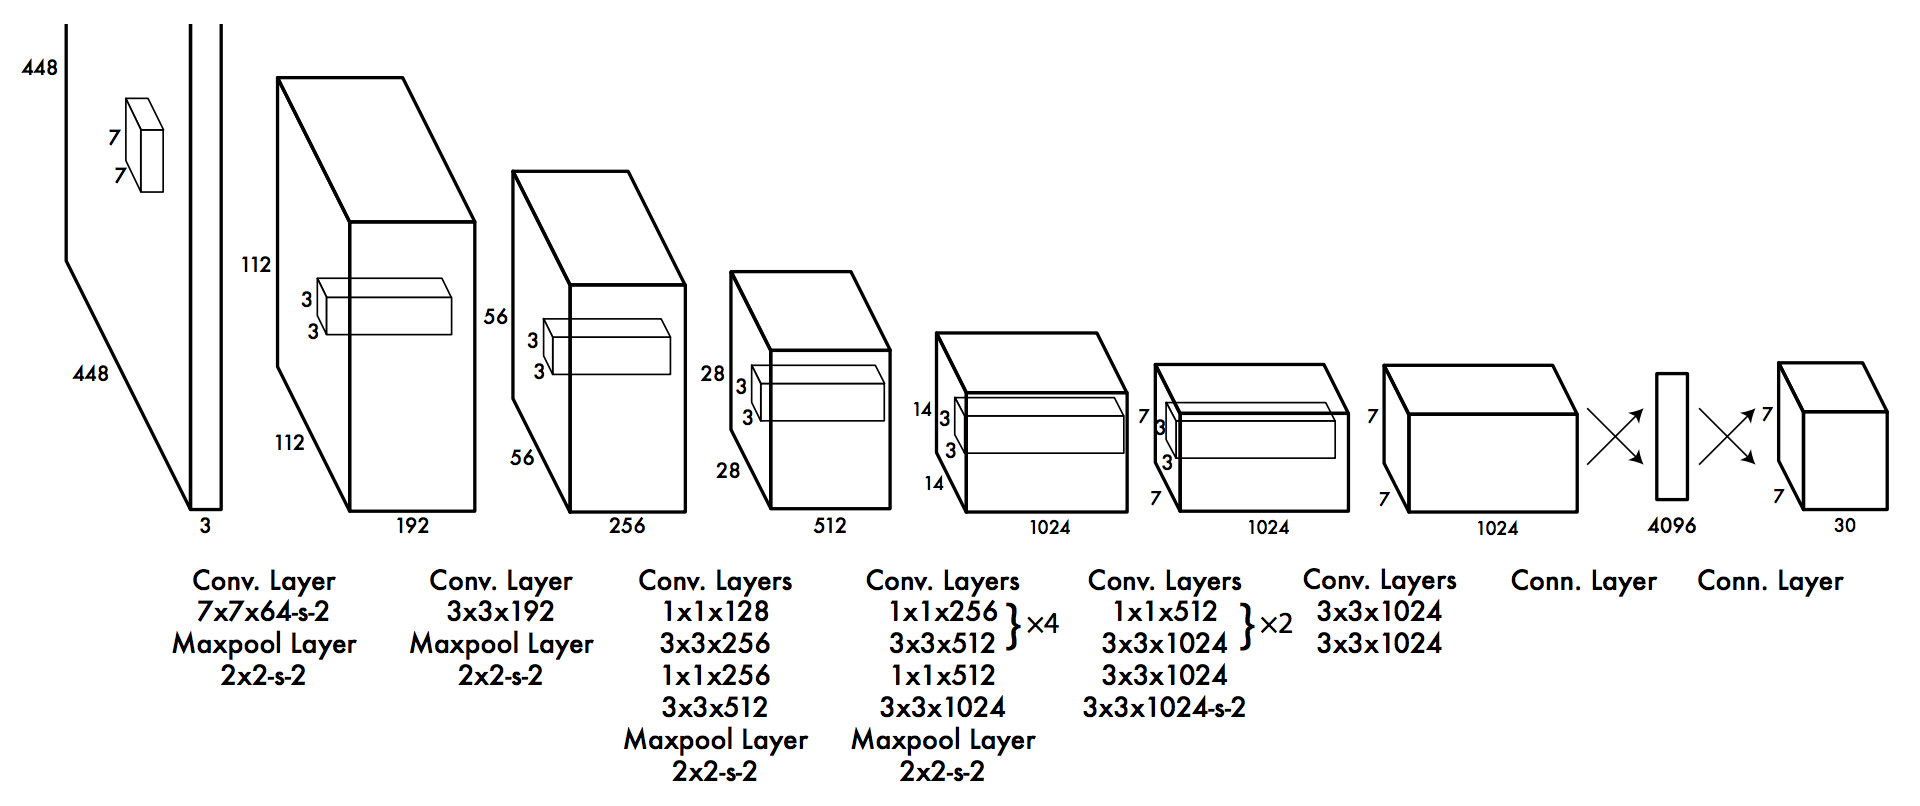
\includegraphics [width=\textwidth]{yoloarch.png}
    \caption{Architecture of YOLO Network \cite{yolo}}
    \label{fig:my_label}
\end{figure}

Figure 4.1 shows the architecture of YOLO. YOLO unify the separate components of object detection into a single neural network. It uses features from the entire image to predict each bounding box.YOLO's system divides the input image into an \(S \times S\)  grid. If the center of an object falls into a grid cell, that grid cell is responsible for detecting that object.

Each grid cell predicts B bounding boxes and confidence scores for those boxes. These confidence scores reflect how confident the model is that the box contains an object and also how accurate it thinks the box is that it predicts. Formally confidence is defined as  
\begin{equation} \label{eq:first2}
  Pr(Object)  \times IOU_{pred} ^ {truth} 
\end{equation}

If no object exists in that cell, the confidence scores should be
zero. Otherwise confidence score will be equal to the intersection over union (IOU) between the predicted box and the ground truth.

Each bounding box consists of 5 predictions: x, y, w, h, and confidence. The (x, y) coordinates represent the center of the box relative to the bounds of the grid cell. The width and height are predicted relative to the whole image. Finally the confidence prediction represents the IOU between the predicted box and any ground truth box.Each grid cell also predicts C conditional class probabilities, 
\begin{equation}
    Pr(Class i | Object)    
\end{equation}


These probabilities are conditioned on the grid cell containing an object. At test time it multiples the conditional class probabilities and the individual box confidence predictions
\begin{equation}\label{eq:firs}
{Pr{(Class i |Object)}} \times {\Pr(Object)} \times IOU_{pred} ^ {truth} = \Pr(Class i) \times IOU_{pred} ^ {truth}
\end{equation}


which gives  class-specific confidence scores for each
box. These scores encode both the probability of that class
appearing in the box and how well the predicted box fits the
object. This is illustrated in the following figure 4.2.


\begin{figure}[H]
\begin{center}
    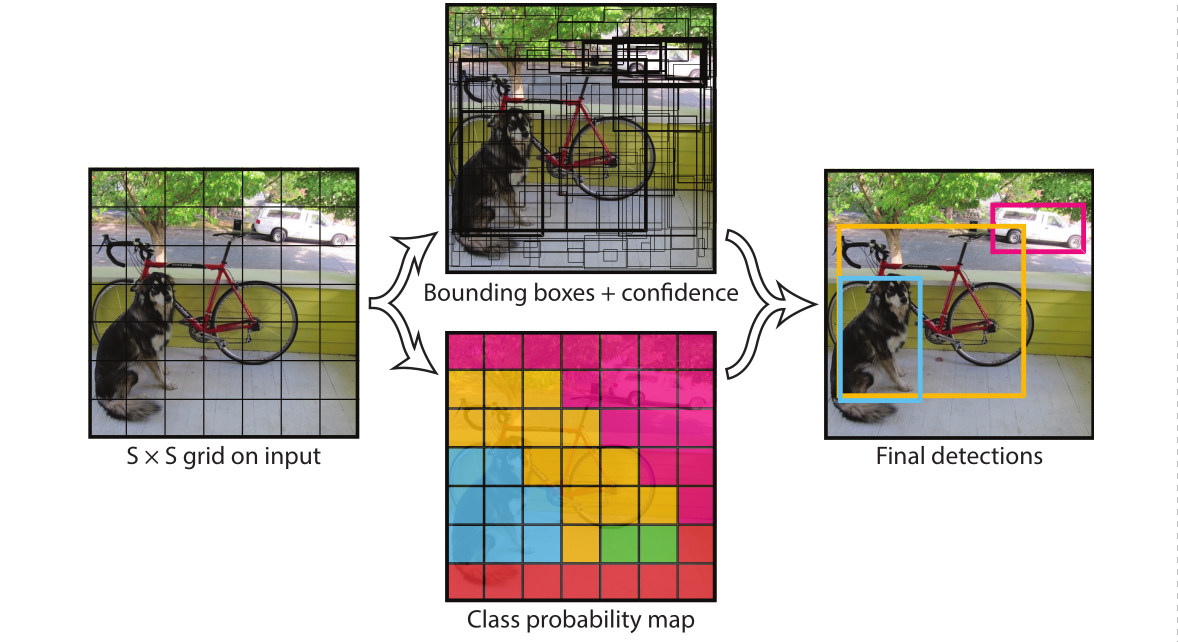
\includegraphics[scale=0.3]{yolo1.png}
    \caption{Object detection as regression problem \cite{yolo}}
\end{center}
\end{figure}
